\chapter{Úvod do problematiky testování materiálů, metody vlastního testování, metoda akustické emise}

\section{Nedestruktivní testování}
V technické praxi jsou struktury namáhány mnoha vnějšími vlivy, čímž se mění jejich materiálové vlastnosti. Například, u laminátových kontrukcí v leteckém průmyslu může vlivem sil nárazu pevnost v tlaku klesnout až o 80\%, i když se materiál jeví jako nepoškozený \cite{Benes_podklad_advances}. 

Pro posouzení stavu materiálu je proto nutné provádět pravidelné testování.
Za účelem stanovení mezních vlastností materiálu jako pevnosti v tlaku, pevnosti v~tahu, lomové houževnatosti, atd., bývá prováděno \ac{DT}. Zahrnuje např. zkoušku tahem, tlakem, nebo ohybem. K těmto zkouškám jsou používány speciální stroje – kladiva, trhačky, ohýbačky, aj. Jak je z názvu přímo patrné, vlastní destruktivní zkoušení končí nevratným poškozením vzorku. 

Pro již hotové konstrukce (např. svařované konstrukce v zámečnické výrobě, betonové pilíře v oblasti stavebnictví) nebo komponenty (hřídele, ozubená kola, kolejnice, atd.) se metody \ac{DT} zpravidla nepoužívají, jelikož by takové zkoušení bylo příliš nákladné. Nabízí se proto použití metod \ac{NDT}. Počátky \ac{NDT} sahají do 19. století, kdy pomocí tzv. akustického poklepového testování byly detekovány praskliny na železničních kolech \cite{ConcretetestingHELAL}.
\section{Metody nedestruktivního testování}
Velká výhoda metod \ac{NDT} spočívá v možnosti zkoušení v kterékoliv části životního cyklu produktu, u některých metod dokonce i v průběhu vykonávání vlastní činnosti výrobku. Díky tomu dostáváme přesné informace o poloze a závažnosti případného defektu ve struktuře materiálu. V současné době na trhu dominuje pět metod nedestruktivního testování – zkoušení magnetickými částicemi, radiografické zkoušení, ultrazvukové zkoušení, zkoušení vířivými proudy a zkoušení metodou akustické emise (dále AE).

Zkoušení magnetickými částicemi spočívá ve vystavení feromagnetických materiálů magnetickému poli. Díky vysoké permeabilitě feromagnetického materiálu se magnetické domény orientují ve~směru působení magnetického pole, tvoří tak souvislé čáry. V případě nespojitosti materiálu dojde k tzv. úniku magnetického pole – čáry v~bodě defektu nebudou spojité. Pro~snadnou viditelnost těchto nespojitostí je použit prášek oxidu železitého, který zmíněné čáry a nespojitosti kopíruje \cite{Gupta_ADVANCES_IN_MATERIALS_AND_PROCESSING_TECHNOLOGIES}. Mezi~limity spadá možnost použití jen pro feromagnetické materiály (železo, kobalt, nikl, ferity, gadolinium, aj.) \cite{Sandeep_Kumar_Dwivedi_NDT}.

Radiografické zkoušení je postup založen na snímání obrázků s využitím radioaktivního zdroje záření. Záření je pohlcováno materiálem a dochází tak k útlumu. Defekty na těchto snímcích lze rozpoznat jako místa s menším útlumem záření \cite{Gupta_ADVANCES_IN_MATERIALS_AND_PROCESSING_TECHNOLOGIES}. Limity představuje nutnost radiační ochrany a nevhodnost použití pro porézní materiály (např. beton, dřevo, sádra, keramiky, kosti aj.) \cite{Sandeep_Kumar_Dwivedi_NDT}

Při zkoušení ultrazvukem je používáno zvukových vln. Piezoelektrický snímač generuje pulzy, které se šíří materiálem. Cestují-li tyto pulzy nepoškozenou, spojitou strukturou, nemění se jejich parametry (především tedy rychlost). Při defektu dochází ke změně rychlosti pulzů.\cite{Gupta_ADVANCES_IN_MATERIALS_AND_PROCESSING_TECHNOLOGIES}. 

Během zkoušení vířivými proudy je kovový materiál umístěn do fluktuujího magnetického pole, které je vytvářeno cívkou. V kovovém materiálu jsou indukovány proudy s vířivou povahou (proto vířivé proudy). Těmito vířivými proudy je vytvořeno sekundární magnetické pole, které ovlivňuje pole cívky. S defektem ve struktuře materiálu dojde tedy ke změně i vířivých proudů, což ovlivní i primární magnetické pole cívky \cite{Gupta_ADVANCES_IN_MATERIALS_AND_PROCESSING_TECHNOLOGIES}. 
\section{Metoda AE. Její výhody, limity}
V případě, že je kovový materiál deformován, uvolňuje se energie ve formě tzv. elastických vln. Tyto elastické vlny jsou vlny vysoké frekvence, které cestují směrem k~povrchu materiálu. Na povrchu tato data sbírají snímače AE. Souřadnice zdrojů AE jsou nejčastěji stanovovány pomocí známého triangulačního algoritmu (podle normy ČSN 14584 \cite{čsn14584}) dle časových diferencí příchodů signálů k jednotlivým snímačům. Tyto snímače jsou na zkoušeném vzorku umístěny v husté síti.

Oproti ultrazvukovému testování je velkou výhodou zkoušení AE možnost nepřetržitého monitorování komponent – při ultrazvukovém zkoušení je potřeba externí zdroj zvuku o vysoké frekvenci. Metodou \ac{AE} se kromě toho nabízí testovat i nekovové nebo porézní materiály a najde tak uplatnění i v netechnických a medicínských oborech (např. diagnostika kostí a kloubů v ortopedii).

Limit metody AE spočívá hlavně v interpretaci dat u komplikovanějších struktur~–~analytické vzorce pro lokalizace zdrojů AE jsou známé jen pro tenkou, izotropní desku \cite{Chlada2009}. Navíc, instalace senzorů na všech požadovaných místech je mnohdy nesnadná. Může tomu tak být z důvodu nepřístupnosti do určitých lokalit konstrukcí (např. některé koutové sváry). Umístění snímačů dokáže mimo to nežádoucím způsobem ovlivnit dynamické vlastnosti konstrukce. %U složitějších struktur probíhá snaha uplatnit umělou neuronovou síť ke zpracování dat.
\section{Postupy použití metody AE u složitějších struktur}%Kompenzace limitů metody AE} 
Z pohledu systémové teorie můžeme testování materiálů metodou AE formulovat dvěma základními způsoby; při~\textbf{dopředné úloze} je stanovována odezva dle známých vstupů (sil nárazů). Nelze-li snadno získat hodnotu vstupu, je formulován problém zpětný – ze~změřené odezvy se dopočítávají hodnoty vstupů. Tento způsob řešení nazveme \textbf{inverzním algoritmem}.

Ve vědeckých studiích bývají tyto inverzní algoritmy k~rekonstrukci působení vnějších sil hojně využívány. Podle implementace již zmíněné inverzní algoritmy jde rozdělit na~techniky založené na~modelech a~techniky založené na~strojovém/hlubokém učení.
\subsection{Techniky založené na modelech}
Při~testování materiálu je odezva (signál AE) zpracovaná předem~vytvořeným modelem. Tento model dle~zpracované odezvy stanovuje vstupní hodnotu a~následně polohu nespojitosti materiálu. Výhoda této techniky spočívá v~nízké výpočetní náročnosti. V používání limituje nutnost tvorby přesného modelu pro přepočty – jak již~bylo výše uvedeno, pro~stanovení vad u~komplikovanějších anizotropních materiálů nejsou známé analytické vzorce, a~je proto velmi obtížné tvořit modely pro testování těchto materiálů. Proto probíhá snaha uplatnit při lokalizaci zdrojů \ac{AE} algoritmy strojového učení.
\subsection{Techniky založené na strojovém učení}
V posledních letech se algoritmy strojového učení stávají velmi vhodnými při~rekonstrukci dat AE – dají se aplikovat i tehdy, když základní mechanismy pro nás nejsou zcela známé a nedovedeme tak správně sestavit model. Nicméně, pro správné uplatnění technik strojového učení představuje omezení nutnost velkého objemu tréninkových dat. 

Neexistuje žádná záruka, že tréninková data získaná pro jednu strukturu přinesou smysluplné výsledky i u struktur odlišných. V posledních letech jsou prozkoumávány proto metody tzv. hlubokého učení (nebo také deep learningu), které umožňují použití dat i v surové podobě. S použitím metod hlubokého učení lze tak interpretovat dokonce i vícerozměrné signály \ac{AE}.

Důležitým algoritmem, na kterém stojí velká většina modelů hlubokého učení, je \textbf{umělá neuronová síť}. Stejně jako ostatní metody hlubokého učení potřebují ke své funkci velký objem tréninkových dat. Studie (například \cite{ghajari}) se v současné době snaží pomocích neuronových sítí identifikovat vnější síly, které způsobují deformační změny na kompozitních panelech. Výhodou neuronových sítí je nepotřeba předchozích znalostí poloh zdrojů deformace. Ve výše uvedené studii jsou aplikovány dvě neuronové sítě – jedna pro deformace o vyšších amplitudách, druhá pro deformace o amplitudách menších.

Navzdory obrovskému potenciálu nejsou umělé neuronové sítě v nelineárních strukturách zcela široce využívány. Způsobují to fakta, že nejčastěji používaná architektura umělých neuronových sítí pracuje s dvourozměrnými vstupy. Prvním parametrem je rozsah datového setu, který je k dispozici k trénování sítě. Druhým je samotný příznak čili měřená data, která neuronové síti přidělíme k učení. Tyto parametry nezahrnují čas, jenž je k rekonstrukci zdroje deformace nezbytný.

Navíc, pro výběr kvalitních příznaků do učící sady je nezbytná lidská expertíza. Tvorba učící sady je poměrně náročná a nelze ji nijak efektivně automatizovat. Při rekonstrukci zdroje deformace mimo jiné představuje problém již výše popsaný u technik založených na modelech – pro získání kvalitních dat je nutné rozmístit senzory v husté síti, a to zhoršuje dynamické parametry konstrukce.

\section{Komerční použití neuronových sítí pro lokalizaci AE}
AE bývá někdy označována jako pasivní ultrazvuk. Ultrazvukové snímače oproti snímačům AE potřebují pro správnou lokalizaci zdroj zvuku o frekvenci, která je vyšší než hranice slyšitelná člověkem (přes 20 kHz). Proto se mnozí výrobci ultrazvukových snímačů a defektoskopů úzce specializují i na diagnostiku metodou AE (např. Olympus). 

Velkým výrobcem, který je kromě jiných metod zaměřen i na AE, je MISTRAS group (patří k nim Physical Acoustic). Menší firma vyrábějící kvalitní a uznávané systémy, snímače a předzesilovače pro testování metodou AE, je Vallen Systeme. Jde tak o velkého konkurenta firmy MISTRAS group. Tito dva největší výrobci mimo jiné ladí a vyvíjejí software pro lokalizaci zdrojů AE pomocí algoritmů neuronových sítí.

% MISTRAS group je provozovatelem všech výše zmíněných metod \ac{DT} – věnují se jak ultrazvukovému testování, testování magnetickými částicemi, i zkoušení materiálů vířivými proudy. Pro testování metodou \ac{AE} provozují vlastní technologickou divizi Physical acoustic. 

%NA ZÁKLADĚ ZPRÁV Z VALLENA A MISTRAS POSOUDIT NÁSLEDUJÍCÍ BODY:
%JAKOU LOKALIZACI ZDROJŮ NABÍZEJÍ (CO 2D/3D DATA)?
%S JAKOU MINIMÁLNÍ VZDÁLENOSTÍ PENTESTU OD SNÍMAČE SE POČÍTÁ?
%JAKÉ TYPY VLN ZVLÁDAJÍ VYHODNOCOVAT?
%//
% Nejnovější generace 32bitového software od společnosti Vallen Systeme pro Windows k analýze zdrojů \ac{AE} se nazývá VisualAE. Součástí tohoto softwaru je stejně tak VisualClass (systém pro tzv. rozpoznávání vzorů) a VisualTR (modul pro digitální filtraci signálu). Veškerá data jsou sbírána podprogramem Acquisition32, který má vysokou spolehlivost a je plně integrován do tohoto systému. Jak VisualClass, tak VisualAE, a stejně tak i VisualTR se tak mohou kdykoliv dostat k libovolnému datasetu.
\subsection{Software od firmy Vallen}
Program VisualClass od společnosti Vallen
 umí rozeznat podobnosti a rozdíly 
 mezi změřenými vlnami AE. Jak je z názvu přímo patrné, umí tato data klasifikovat~–~každé vlně přidělí určité číslo třídy. V každé z těchto přidělených tříd klasifikuje podobnost se vzorovými 
daty. Funkcí, která představuje míru podobnosti mezi vlastní změřenou vlnou a vzorem, je poměr vzdáleností. Čím nižší je poměr vzdáleností, tím lépe odpovídá aktuální průběh přidělené třídě. Výsledky těchto klasifikátorů mohou být pro každý dílčí detekovaný zásah v programu VisualAE (program od společnosti Vallen pro analýzu dat AE. Zpracovává jak dvojrozměrná, tak trojrozměrná data, počítá hodnoty nejistot měření, atd.) spojeny s odpovídajícími parametry. Klasifikované výsledky lze tak i statisticky zpracovat.

Výše zmíněný klasifikátor (čili kritérium, kterým jsou vlnové průběhy přidělovány do tříd) lze chápat jako výsledek procesu učení. V rámci procesu učení je brán určitý počet datových (učících) sad. Byla-li data vybrána uživatelem, hovoří se o \textbf{řízeném učení} (supervised learning). Pokud byly tyto sady vybrány automaticky nějakým výkonným algoritmem shlukování (tzv. clustering), jde potom o učení \textbf{neřízené} (unsupervised learning).

Průběhy uvedené na obrázcích \ref{fig:visualclass_3cm}, \ref{fig:visualclass_6cm} a \ref{fig:visualclass_11cm} byly změřeny shodným senzorem, zpracování proběhlo softwarem od VisualClass. Vzdálenost zdroje AE od snímače jsou 3, 6 a 11 cm. Pro každou z níže uvedených pozic bylo generováno deset pulzů.
\begin{figure}[!h]
    \centering
    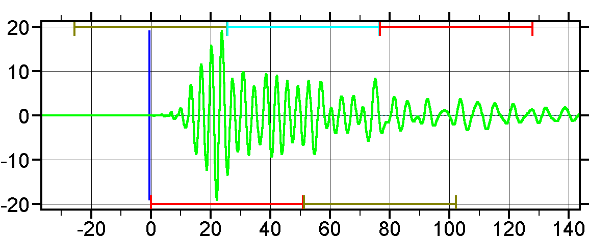
\includegraphics[width=0.7\linewidth]{obrazky/visualclass_3cm.png}
    \caption{Signál akustické emise pro vzdálenost senzoru od zdroje 3 cm \cite{vallen_visual_class}}
    \label{fig:visualclass_3cm}
\end{figure}

\begin{figure}[!h]
    \centering
    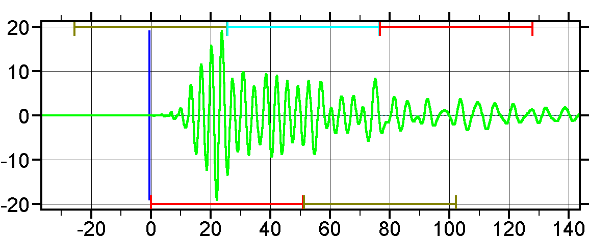
\includegraphics[width=0.7\linewidth]{obrazky/visualclass_3cm.png}
    \caption{Signál akustické emise pro vzdálenost senzoru od zdroje 6 cm \cite{vallen_visual_class}}
    \label{fig:visualclass_6cm}
\end{figure}

\begin{figure}[!h]
    \centering
    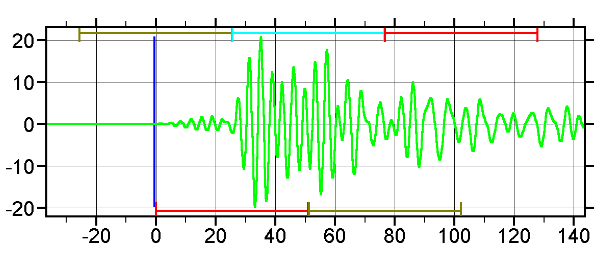
\includegraphics[width=0.7\linewidth]{obrazky/visualclass_11cm.png}
    \caption{Signál akustické emise pro vzdálenost senzoru od zdroje 11 cm \cite{vallen_visual_class}}
    \label{fig:visualclass_11cm}
\end{figure}
Pro takto změřené signály
 AE potom VisualClass dokáže zobrazovat 
 spektra krátkodobé frekvenční analýzy 
 (zobrazení spektrogramu). 
 Příklad frekvenční analýzy pro průběh uvedený na~obrázku \ref{fig:visualclass_3cm} je uveden na~obrázku \ref{fig:vallen_frekvencni_analyza}. 
\begin{figure}[!h]
    \centering
    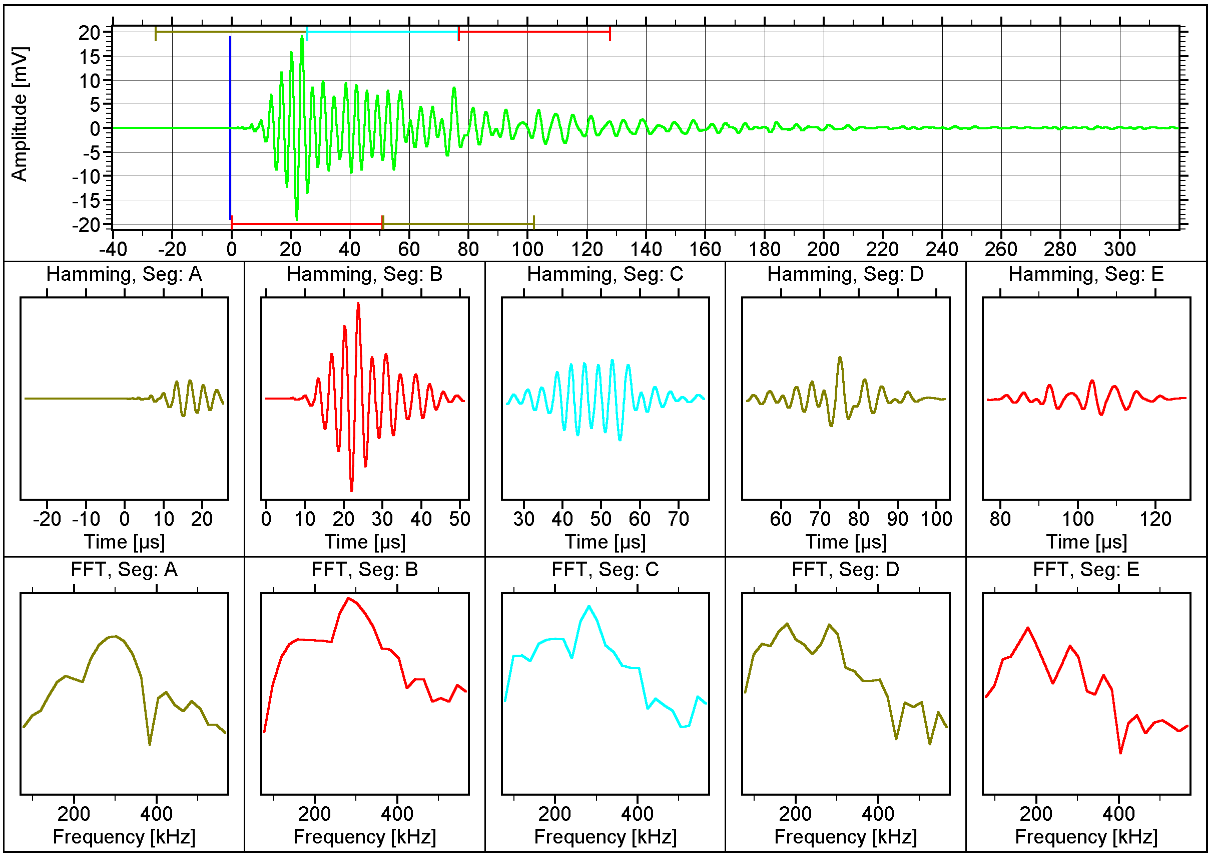
\includegraphics[width=0.75\linewidth]{visual_class_spectral_analysis.png}
    \caption{Frekvenční analýza pro signál AE z obrázku \ref{fig:visualclass_3cm} \cite{vallen_visual_class}}
    \label{fig:vallen_frekvencni_analyza}
\end{figure}
Jak lze na obrázku 
\ref{fig:vallen_frekvencni_analyza} vidět, 
je signál rozdělen na~malé časové segmenty. 
Každý z těchto časových segmentů je zobrazen 
pomocí Hammingova okna, abychom se 
vyhnuli strmým hranám oken. 
Tyto hrany totiž zkreslují skutečné průběhy.
Následně se pro každý v horní části
obrázku \ref{fig:vallen_frekvencni_analyza} 
vyznačený časový segment
pomocí algoritmu FFT stanoví vlastní spektrum, 
jak lze vidět ve spodní části obrázku 
\ref{fig:vallen_frekvencni_analyza}.

\subsection{Software od firmy Physical acoustic (MISTRAS)}

\section{Případný vývoj}







